% SC4063 --- Chapter 2: Firewalls and Network Segmentation (0->100)
\chapter{Firewalls and Network Segmentation}\label{ch:firewall}
\sloppy

\begin{quote}
\emph{``A firewall is a policy made of packets.''} --- If the network is a
city, the firewall is the checkpoint that asks every car for papers and
decides, by rule, who passes and who is turned away.
\end{quote}

\noindent\fbox{\parbox{\dimexpr\linewidth-2\fboxsep-2\fboxrule}{%
\textbf{From zero: packets first.} We start from a single IP header, add one
rule, then a table, then state, then an application parser. Every concept is
built incrementally: intuition (checkpoint) $\to$ header fields $\to$ rule
$\to$ connection table $\to$ segmented topology. No prior firewall knowledge
assumed.}}
\vspace{0.4em}

\section*{Learning Outcomes}
After this chapter you will be able to:
\begin{enumerate}[label=(L\arabic*)]
    \item distinguish packet-filter, stateful, proxy, and NGFW generations;
    \item write and audit an \texttt{iptables}/\texttt{nftables} rule set and explain first-match semantics;
    \item explain conntrack and the TCP state machine for stateful filtering;
    \item design a screened-subnet DMZ and reason about micro-segmentation;
    \item evaluate firewall limits (encryption, insider, covert channels) and pair with IDS.
\end{enumerate}

% ============================================================
\section{What a Firewall Sees}\label{sec:what-firewall-sees}
A flow is the 5-tuple
$(\text{srcIP},\text{dstIP},\text{srcPort},\text{dstPort},\text{proto})$.
A firewall policy is a function $f$: 5-tuple $\to$ \{allow, deny, log\}.
The wire does not provide intent, only headers and perhaps a payload. Each
generation of firewall sees strictly more context at higher cost.

\begin{figure}[h]\centering
\resizebox{\linewidth}{!}{%
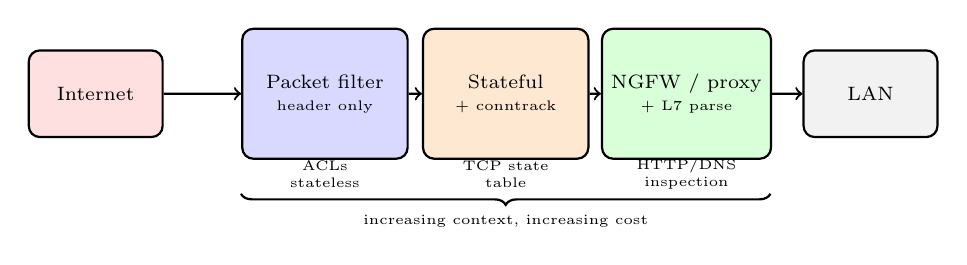
\begin{tikzpicture}[scale=0.82, every node/.style={font=\scriptsize}]
\node[draw,thick,fill=red!12,rounded corners,minimum width=1.7cm,minimum height=1.1cm] (inet) at (0,1.7) {Internet};
\node[draw,thick,fill=blue!15,rounded corners,minimum width=2.1cm,minimum height=1.65cm,align=center] (pf) at (3.55,1.7) {Packet filter\\\tiny header only};
\node[draw,thick,fill=orange!18,rounded corners,minimum width=2.1cm,minimum height=1.65cm,align=center] (st) at (6.35,1.7) {Stateful\\\tiny + conntrack};
\node[draw,thick,fill=green!15,rounded corners,minimum width=2.1cm,minimum height=1.65cm,align=center] (app) at (9.15,1.7) {NGFW / proxy\\\tiny + L7 parse};
\node[draw,thick,fill=gray!10,rounded corners,minimum width=1.7cm,minimum height=1.1cm] (lan) at (12.0,1.7) {LAN};
\draw[->,thick] (inet) -- (pf); \draw[->,thick] (pf) -- (st); \draw[->,thick] (st) -- (app); \draw[->,thick] (app) -- (lan);
\node[font=\tiny,align=center] at (3.55,0.45) {ACLs\\stateless};
\node[font=\tiny,align=center] at (6.35,0.45) {TCP state\\table};
\node[font=\tiny,align=center] at (9.15,0.45) {HTTP/DNS\\inspection};
\draw[decorate,decoration={brace,mirror,amplitude=4pt},thick] (2.25,0.15) -- (10.45,0.15) node[midway,below=4pt,font=\tiny] {increasing context, increasing cost};
\end{tikzpicture}}%
\caption{Firewall generations as a pipeline. Packet filters match headers; stateful adds a connection table; NGFW/proxy terminates and parses the application.}
\label{fig:fw-generations}
\end{figure}

\begin{description}[leftmargin=1.2em,itemsep=0.35em]
    \item[Packet filter (stateless)] Matches header fields only. Rule
    \texttt{deny tcp any any eq 23} blocks Telnet anywhere. Fast, cheap, but
    cannot tell whether a packet belongs to an existing flow; return traffic
    needs a broad reverse rule that attackers abuse.
    \item[Stateful firewall] Keeps a \emph{state table} of active flows (SYN seen,
    ESTABLISHED, RELATED). Return SYN-ACK is allowed only if a matching SYN
    is in the table, blocking unsolicited inbound TCP and spoofed ACKs. This is
    \texttt{conntrack} in Linux.
    \item[Application proxy / NGFW] Terminates the connection, parses the
    application (HTTP, DNS, TLS SNI), and enforces content policy:
    \texttt{deny http POST to /admin from !corp}, strip ActiveX, block DNS
    tunnelling. Highest visibility, highest latency and certificate cost. A WAF
    is this idea specialised to HTTP.
\end{description}

\begin{example}[Rule order matters]\label{ex:order}
Default-deny with rules in order: (1) \texttt{allow tcp 10.0.0.0/8 any eq 443},
(2) \texttt{allow tcp any 10.0.0.5 eq 80}, (3) \texttt{deny ip any any}.
A packet to \texttt{10.0.0.5:80} matches (2); placed below (3) it would be
dropped. First-match semantics and shadowing cause most firewall outages.
\texttt{iptables -L -n --line-numbers} audits order.
\end{example}

% ============================================================
\section{Stateful Filtering and Conntrack}\label{sec:stateful}
 Stateless ``allow \texttt{any any established}'' lets an attacker reach an
internal service by setting the ACK bit. Stateful fixes it: only packets
belonging to a known connection pass.

\begin{definition}[State table entry]\label{def:conntrack}
An entry keys on the 5-tuple plus TCP state \{NEW, ESTABLISHED, RELATED,
INVALID\}, timeout, and counters. On outbound SYN, insert NEW; on matching
SYN-ACK, promote to ESTABLISHED; on FIN/RST, schedule expiry. The reverse
direction inherits permission from the forward entry.
\end{definition}

\begin{figure}[h]\centering
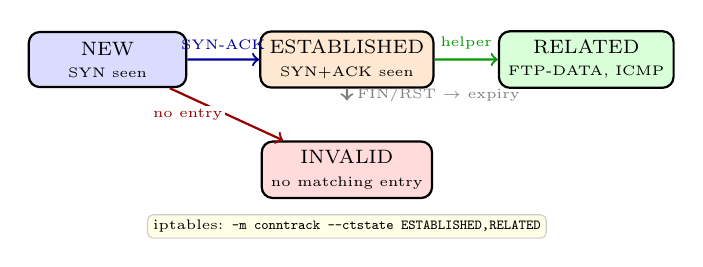
\begin{tikzpicture}[scale=0.80, every node/.style={font=\scriptsize},
  st/.style={draw,thick,rounded corners=4pt,minimum width=2.0cm,minimum height=0.70cm,align=center}]
\node[st,fill=blue!14] (new) at (0,1.2) {NEW\\\tiny SYN seen};
\node[st,fill=orange!18] (est) at (3.8,1.2) {ESTABLISHED\\\tiny SYN+ACK seen};
\node[st,fill=green!15] (rel) at (7.6,1.2) {RELATED\\\tiny FTP-DATA, ICMP};
\node[st,fill=red!14] (inv) at (3.8,-0.55) {INVALID\\\tiny no matching entry};
\draw[->,thick,blue!60!black] (new) -- (est) node[midway,above,font=\tiny] {SYN-ACK};
\draw[->,thick,green!60!black] (est) -- (rel) node[midway,above,font=\tiny] {helper};
\draw[->,thick,red!60!black] (new) -- (inv) node[midway,left,font=\tiny,fill=white,inner sep=1pt] {no entry};
\draw[->,thick,gray] (est) -- ++(0,-0.65) node[midway,right,font=\tiny] {FIN/RST $\to$ expiry};
\node[font=\tiny,fill=yellow!10,rounded corners=2pt,inner sep=2pt,draw=gray!40] at (3.8,-1.45) {iptables: \texttt{-m conntrack --ctstate ESTABLISHED,RELATED}};
\end{tikzpicture}
\caption{Conntrack state machine (simplified). Only ESTABLISHED/RELATED return traffic is allowed, blocking spoofed ACKs that stateless filters admit.}
\label{fig:conntrack}
\end{figure}

Linux implements this as \texttt{nf\_conntrack}. Every NAT translation also
consumes a conntrack entry, so table exhaustion is a DoS vector (Ch.~5).

\begin{lstlisting}[language=bash,caption={Stateful iptables: default-deny with conntrack.},label={lst:iptables}]
# Default deny
iptables -P INPUT DROP
iptables -P FORWARD DROP
iptables -P OUTPUT DROP
# Allow loopback and established return traffic
iptables -A INPUT  -i lo -j ACCEPT
iptables -A INPUT  -m conntrack --ctstate ESTABLISHED,RELATED -j ACCEPT
# Allow outbound 80/443 and DNS to 8.8.8.8, log the rest
iptables -A OUTPUT -o eth0 -p tcp --dport 80  -m conntrack --ctstate NEW -j ACCEPT
iptables -A OUTPUT -o eth0 -p tcp --dport 443 -m conntrack --ctstate NEW -j ACCEPT
iptables -A OUTPUT -o eth0 -p udp --dport 53 -d 8.8.8.8 -j ACCEPT
iptables -A OUTPUT -j LOG --log-prefix "DROP-OUT: "
# Shadowed-rule audit: insert a broad deny before a narrow allow and watch it break
\end{lstlisting}

\texttt{nftables} replaces the four tables with one rule set and supports sets
and intervals, but the semantics (first match, conntrack) are identical.

% ============================================================
\section{Segmentation: DMZ and Beyond}\label{sec:segment}
One firewall is one failure. A \emph{screened subnet} places public servers
in a DMZ between two firewalls: outer allows Internet$\to$DMZ on 80/443,
inner allows DMZ$\to$LAN only for needed flows (app$\to$DB on 5432).
Compromise of the DMZ does not directly expose the LAN.

\begin{figure}[h]\centering
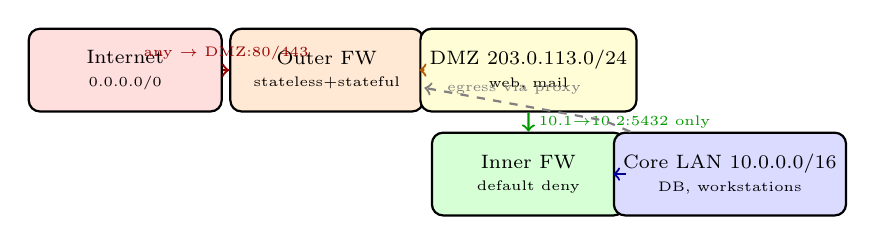
\begin{tikzpicture}[scale=0.80, every node/.style={font=\scriptsize},
  net/.style={draw,thick,rounded corners=4pt,minimum width=2.45cm,minimum height=1.05cm,align=center}]
\node[net,fill=red!13] (inet) at (0,1.70) {Internet\\\tiny 0.0.0.0/0};
\node[net,fill=orange!17] (fw1) at (3.2,1.70) {Outer FW\\\tiny stateless+stateful};
\node[net,fill=yellow!16] (dmz) at (6.4,1.70) {DMZ 203.0.113.0/24\\\tiny web, mail};
\node[net,fill=green!16] (fw2) at (6.4,0.05) {Inner FW\\\tiny default deny};
\node[net,fill=blue!14] (lan) at (9.6,0.05) {Core LAN 10.0.0.0/16\\\tiny DB, workstations};
\draw[->,thick,red!60!black] (inet) -- (fw1) node[midway,above,font=\tiny] {any $\to$ DMZ:80/443};
\draw[->,thick,orange!70!black] (fw1) -- (dmz);
\draw[->,thick,green!60!black] (dmz) -- (fw2) node[midway,right,font=\tiny] {10.1$\to$10.2:5432 only};
\draw[->,thick,blue!60!black] (fw2) -- (lan);
\draw[->,thick,gray,dashed] (lan) -- ++(-2.0,0.85) -- (fw1) node[midway,above,font=\tiny] {egress via proxy};
\end{tikzpicture}
\caption{Screened-subnet DMZ. Two firewalls enforce least privilege per hop. Egress from LAN is proxied and logged, not routed directly.}
\label{fig:dmz}
\end{figure}

Modern networks push further: \emph{micro-segmentation} treats every workload
as its own zone (Kubernetes NetworkPolicy, host firewalls, identity-aware
proxies). NAT hides private addresses but is not a security control; a
misconfigured NAT that hairpins or forwards ports reopens the surface.

\begin{lstlisting}[language=Python,caption={Toy stateless firewall: first-match ACL evaluation.},label={lst:fw-sim}]
rules = [("allow","10.0.0.0/8","any",443), ("allow","any","10.0.0.5",80),
         ("deny","any","any","any")]  # order matters
import ipaddress
def match(pkt, rule):
    _, src, dst, dport = rule
    def net_match(net, ip):
        return net=="any" or ipaddress.ip_address(ip) in ipaddress.ip_network(net)
    return net_match(src, pkt["src"]) and net_match(dst, pkt["dst"]) and (dport=="any" or pkt["dport"]==dport)

pkt = {"src":"8.8.8.8","dst":"10.0.0.5","dport":80}
for r in rules:
    if match(pkt, r):
        print(r[0], "by", r); break  # first match wins
\end{lstlisting}

Firewalls are blind to encrypted payloads, insider traffic, and covert
channels (DNS tunnelling, ICMP exfil). That is why every firewall deployment
is paired with IDS/IPS (Ch.~3) on a decrypted copy and with host controls.
A firewall that logs nothing is a firewall that cannot be audited.

\begin{remark}[Egress matters more]\label{rem:egress}
Ingress rules block outsiders; egress rules catch insiders and compromised
hosts calling home. An allow-list for outbound (only proxy $\to$ 80/443, DNS
to vetted resolvers) stops most command-and-control without touching a single
ingress rule.
\end{remark}

% ============================================================
\section{Exercises}\label{sec:ch02-exercises}
\begin{enumerate}[label=E2.\arabic*, leftmargin=*, itemsep=0.6em]
    \item \textbf{ACL audit.} Write a default-deny rule set for \texttt{203.0.113.10}
    that allows inbound 443/80 from anywhere, outbound DNS (UDP~53) to
    \texttt{8.8.8.8}, and blocks Telnet (23) explicitly. Identify one shadowed
    rule if the deny-all is moved to the top.
    \item \textbf{Stateless vs.\ stateful.} A stateless filter has \texttt{allow tcp any any established}.
    Show how an attacker reaches an internal service on 8080 by setting ACK.
    What exact conntrack entry after a legitimate SYN would a stateful firewall
    check to block that attack?
    \item \textbf{DMZ design.} Place a 3-tier app (WAF, app servers, DB) in a
    screened subnet. For each firewall, list allowed 5-tuples. Explain why the
    DB must have no route to the Internet even via NAT.
    \item \textbf{iptables lab.} Translate the rule set in Listing~\ref{lst:iptables}
    to \texttt{nftables} syntax. Add a rate-limit of 20 new SSH connections per
    minute with \texttt{--limit} and explain where it mitigates brute force.
    \item \textbf{Limits of firewalls.} Give one attack that a correctly configured
    NGFW still misses for each of: (a) encrypted payload, (b) insider, (c) DNS
    covert channel. For each, name the complementary control (IDS, DLP, DNS filter).
\end{enumerate}

\section*{Chapter Notes}
Firewalls originate from Cheswick--Bellovin (1994); stateless vs.\ stateful is
codified in Chapman--Zwicky (1995). Linux conntrack and \texttt{iptables}/
\texttt{nftables} are documented in \texttt{netfilter.org} and Michael Rash's
\texttt{Netfilter} references. NGFW/WAF trade-offs follow NSS Labs tests and
NIST SP~800-41 Rev~1. DMZ and segmentation patterns are in NIST SP~800-41 and
NSA's network segmentation guidance; micro-segmentation aligns with NIST
SP~800-207 (Zero Trust).
% End of Chapter 2
